% =====================================================================
%  Dokumentace projektu IFJ26 (IFJ + IAL 2026/2027)
%
%  Pravidla ze zadání (sekce 4 a 5), na která je třeba myslet:
%   - Text dokumentace píšeme SAMI. AI je zakázáno použít na generování
%     i úpravu textu dokumentace a na přípravu gramatiky, LL tabulky,
%     automatu a precedenční tabulky. Takže se omlouvám za moje překlepy a %     nedostatek čárek.
%   - Dokumentace má být velmi stručná. Projekt nepředstavujeme ani
%     nevysvětlujeme, co dělá -- rovnou píšeme, JAK jsme to udělali,
%     případně co neumí.
%   - Jako vždy nekopírovat úryvky kódu. Identifikátory sázet \texttt{}.
%   - Diagramy a tabulky musí být čitelné po vytištění na A4. Testuji KA.
%   - Hodnotí se obsah, stylistika, pochopitelnost, struktura a sazba.
%   - Zdroják se verzuje v gitu s projektem, ale NEDÁVAT do archivu.
%
%  Před odevzdáním: \TODOfalse (níže) skryje všechny žluté poznámky
%  a v logu nesmí zůstat žádné "TODO"!!!
% =====================================================================
\documentclass[11pt,a4paper]{article}

% --- kódování, jazyk, písmo ------------------------------------------
\usepackage[utf8]{inputenc}
\usepackage[T1]{fontenc}
\usepackage[czech]{babel}
\usepackage{lmodern}
\usepackage{microtype}
\usepackage{csquotes}            % \enquote{...} = české uvozovky

% --- sazba stránky ----------------------------------------------------
\usepackage[a4paper,left=2.5cm,right=2.5cm,top=2.5cm,bottom=2.5cm]{geometry}
\usepackage{parskip}            % odstavce oddělené mezerou, bez odsazení

% --- obrázky, tabulky -------------------------------------------------
\usepackage{graphicx}
\usepackage{float}
\usepackage[section]{placeins}  % obrázky nepřetečou za konec své sekce
\usepackage{booktabs}
\usepackage{array}
\usepackage{multirow}
\usepackage{longtable}
\usepackage{pdflscape}          % LL tabulka na šířku
\usepackage[table]{xcolor}
\usepackage{caption}
\captionsetup{justification=centering}
\usepackage{subcaption}
% uvolnění limitů plovoucích obrázků a pevné rozestupy bez gumových děr
\renewcommand{\topfraction}{0.9}
\renewcommand{\bottomfraction}{0.85}
\renewcommand{\textfraction}{0.07}
\renewcommand{\floatpagefraction}{0.75}
\makeatletter
\setlength{\@fptop}{8pt}
\setlength{\@fpsep}{18pt}
\setlength{\@fpbot}{0pt plus 1fil}
\makeatother
\usepackage{tikz}
\usetikzlibrary{positioning,arrows.meta,shapes.geometric,babel} % babel: czech dělá - aktivní

% --- seznamy, odkazy, citace -----------------------------------------
\usepackage{enumitem}
\usepackage{amsmath,amssymb}
\usepackage[hidelinks,unicode]{hyperref}
\usepackage{url}

% --- vlastní makra ----------------------------------------------------
% =====================================================================
%  Pomocná makra
% =====================================================================

% --- poznámky "co sem napsat" ----------------------------------------
% \TODOtrue  = poznámky jsou vidět (žlutě zvýrazněný text)
% \TODOfalse = poznámky zmizí (PŘED ODEVZDÁNÍM)
\newif\ifTODO
\TODOfalse

% zvýraznění textu přes více řádků (soulutf8 = soul s podporou UTF-8)
\usepackage{soulutf8}
\sethlcolor{yellow!45}
% příkazy, které se v \hl{} smí objevit (berou se jako celek)
\soulregister\texttt7
\soulregister\textbf7
\soulregister\emph7
\soulregister\ref7
\soulregister\dots0
\soulregister\soubor7
\soulregister\fce7
\soulregister\tok7

\newcommand{\TODO}[1]{%
  \ifTODO
    \par\noindent{\small\hl{\textbf{TODO:} #1}}\par
    \typeout{TODO: zbyva vyplnit poznamku v dokumentaci}%
  \fi}
\newcommand{\TODOinline}[1]{%
  \ifTODO{\small\hl{#1}}\typeout{TODO: inline}\fi}

% --- titulní strana --------------------------------------------------
% \clen{Jméno Příjmení}{xlogin00}{VUT ID}{procenta}
\newcommand{\clen}[4]{#1 & \texttt{#2} & #3 & #4\,\% \\}
\newcommand{\vedouci}[4]{\textbf{#1} & \texttt{\textbf{#2}} & \textbf{#3} & \textbf{#4\,\%} \\}

% --- identifikátory, soubory -----------------------------------------
\newcommand{\soubor}[1]{\texttt{#1}}     % \soubor{lexer.c}
\newcommand{\fce}[1]{\texttt{#1()}}       % \fce{lexer_next} -> lexer_next()
\newcommand{\tok}[1]{\texttt{#1}}         % \tok{TOKEN\_IDENTIFIER}

% --- gramatika -------------------------------------------------------
\newcommand{\nt}[1]{\ensuremath{\langle}\textit{#1}\ensuremath{\rangle}} % neterminál
\newcommand{\tm}[1]{\texttt{#1}}          % terminál
\newcommand{\eps}{\ensuremath{\varepsilon}}
\newcommand{\pravidlo}{\ensuremath{\rightarrow}}

% pravidlo: \item ... \label{r:x}, v LL tabulce \ref{r:x}
\newlist{gramatika}{enumerate}{1}
\setlist[gramatika]{label=\arabic*.,ref=\arabic*,itemsep=0pt,leftmargin=2.5em}

% --- konečný automat (TikZ) -----------------------------------------
% konvence IFJ: koncový stav = dvojitý kruh, "+" = jeden ze znaků
\usetikzlibrary{automata}
\tikzset{
  ka/.style={
    >={Stealth[round,length=2mm]}, shorten >=1pt, auto,
    font=\footnotesize,
    every state/.style={draw, thick, minimum size=7.5mm, inner sep=0pt,
                        font=\small, fill=white},
    every edge/.style={draw, ->, thin},
    every edge quotes/.style={font=\footnotesize, inner sep=1.5pt},
    initial text={}, initial distance=6mm,
  },
  % souřadnice = pixely původních PNG z diagrams.io
  px/.style={x=0.0098cm, y=-0.0115cm},
  hrana/.style={->, >={Stealth[round,length=2mm]}, shorten >=1pt,
                rounded corners=4pt},
  lbl/.style={font=\footnotesize, inner sep=1.5pt},
  tok/.style={font=\scriptsize\ttfamily, text=black!70},
  pozn/.style={font=\scriptsize\itshape, text=black!60},
}
% symboly v popiscích hran (babel czech dělá z " aktivní znak!)
\newcommand{\kaUv}{\texttt{\textquotedbl}}            % "
\newcommand{\kaBs}{\texttt{\textbackslash}}           % \
\newcommand{\kaPod}{\texttt{\_}}                      % _
\newcommand{\kaPis}{\texttt{a..z}\,+\,\texttt{A..Z}}  % písmena
\newcommand{\kaCis}{\texttt{0..9}}                    % číslice
\newcommand{\kaKrome}[1]{\ensuremath{\Sigma-\{}#1\ensuremath{\}}}

% --- precedenční tabulka -------------------------------------------
\newcommand{\shift}{\ensuremath{<}}
\newcommand{\reduce}{\ensuremath{>}}
\newcommand{\equal}{\ensuremath{=}}
\newcommand{\chyba}{}


% =====================================================================
%  ÚDAJE NA TITULNÍ STRANU -- vyplnit jen tady
% =====================================================================
\newcommand{\tymID}{xpopovd00}                % login vedoucího = ID týmu
\newcommand{\varianta}{vv-BVS}                 % podle registrace v IS VUT
% musí sedět se souborem rozsireni
\newcommand{\rozsireni}{\texttt{FUNEXP}, \texttt{VALMEM}, \texttt{BOOLTHEN}, \texttt{CONTROL}}
\newcommand{\repozitar}{\url{https://github.com/tadeas-z/ifj}}

\begin{document}

% =====================================================================
%  TITULNÍ STRANA
% =====================================================================
\begin{titlepage}
  \centering
  % logo FIT VUT
  
\includegraphics[width=0.6\linewidth]{obrazky/FIT_barevne_CMYK_CZ.pdf}\par
  \vspace{3.5cm}

  {\Huge\bfseries Implementace překladače\\[0.3em]
   imperativního jazyka IFJ26\par}
  \vspace{1em}
  {\Large Dokumentace k~projektu IFJ a IAL 2026/2027\par}
  \vspace{2.5cm}

  {\large Tým \texttt{\tymID}, varianta \textbf{\varianta}\par}
  \vspace{1.5cm}

  % \clen / \vedouci{jméno}{login}{VUT ID}{procenta}, podle rozdeleni
  \begin{tabular}{l l l r}
    \toprule
    \textbf{Jméno} & \textbf{Login} & \textbf{VUT ID} & \textbf{Body} \\
    \midrule
    \vedouci{Dušan Popović}{xpopovd00}{282582}{25}
    \clen{Marek Záchenský}{xzachem00}{270480}{25}
    \clen{Adam Zatloukal}{xzatloa01}{282559}{25}
    \clen{Tadeáš Zonyga}{xzonygt00}{282294}{25}
    \bottomrule
  \end{tabular}
  \par\vspace{1.5cm}

  \begin{tabular}{r l}
    Implementovaná rozšíření: & \rozsireni \\
    Repozitář:                & \repozitar \\
  \end{tabular}

  \vfill
  {\large \today\par}   % datum překladu
\end{titlepage}

\tableofcontents
\newpage

% =====================================================================
%  OBSAH (pořadí podle sekce 5 zadání)
% =====================================================================
% =====================================================================
%  Rozdělení práce
% =====================================================================
\section{Rozdělení práce}\label{sec:tym}

\begin{description}[style=nextline]
  % git: src/parser, tests/parser
  \item[Dušan Popović]
    LL parser programu a příkazů, precedenční analýza výrazů,
    syntaktické chyby (kód 2), testy parseru.

  % git: src/codegen, tests/e2e, tests/codegen
  \item[Marek Záchenský]
    generování IFJcode26, vestavěné funkce, \texttt{main}, Makefile
    a propojení všech částí, testy generátoru, end-to-end testy.

  % git: src/semantic, src/symtable, src/common, .clang-format
  \item[Adam Zatloukal]
    tabulka symbolů (vv-BVS), AST, dynamické pole, společné typy
    a chybové kódy (\texttt{comp\_error.h}), sémantické kontroly
    (kódy 3--7 a 10), testy v~GoogleTestu.

  % git: src/lexer, tests/lexer, diagramy lexeru
  \item[Tadeáš Zonyga]
    konečný automat, tokeny (\texttt{token.h}), čísla, stringy
    a víceřádkové stringy, komentáře, odsazení a logické řádky,
    lexikální chyby (kód 1), testy lexeru.
\end{description}

% =====================================================================
%  Spolupráce, testování, formátování
% =====================================================================
\section{Spolupráce a vývojový proces}\label{sec:spoluprace}

\subsection{Spolupráce, code review a schvalování PR}
Vývoj probíhal na GitHubu, kde každý člen týmu pracoval ve vlastní větvi.
Snažili jsme se vytvářet menší commity, po kterých byl projekt stále
přeložitelný. Každý pull request před začleněním do větve \texttt{main}
kontroloval a schvaloval jiný člen týmu. Ke komunikaci jsme využívali
Discord, kde jsme pravidelně probírali průběh vývoje a případné problémy.

\subsection{Testování}
Pro testování tabulky symbolů, AST a sémantické analýzy jsme využili
GoogleTest. Lexer má vlastní regresní testy v~\texttt{test\_lexer.c}, které
ověřují typy tokenů, jejich pozice, lexémy, hraniční případy a chybové
vstupy. Testovali jsme také rozšíření jazyka, správu paměti a funkčnost
celého překladače.

\subsection{Formátování kódu}
Pro jednotné formátování kódu jsme používali \texttt{clang-format} se stylem
WebKit, jehož konfigurace je součástí repozitáře v~souboru
\soubor{.clang-format}.

% =====================================================================
%  Architektura
% =====================================================================
\section{Architektura překladače}\label{sec:architektura}

\begin{figure}[H]
  \centering
  % až bude schéma: 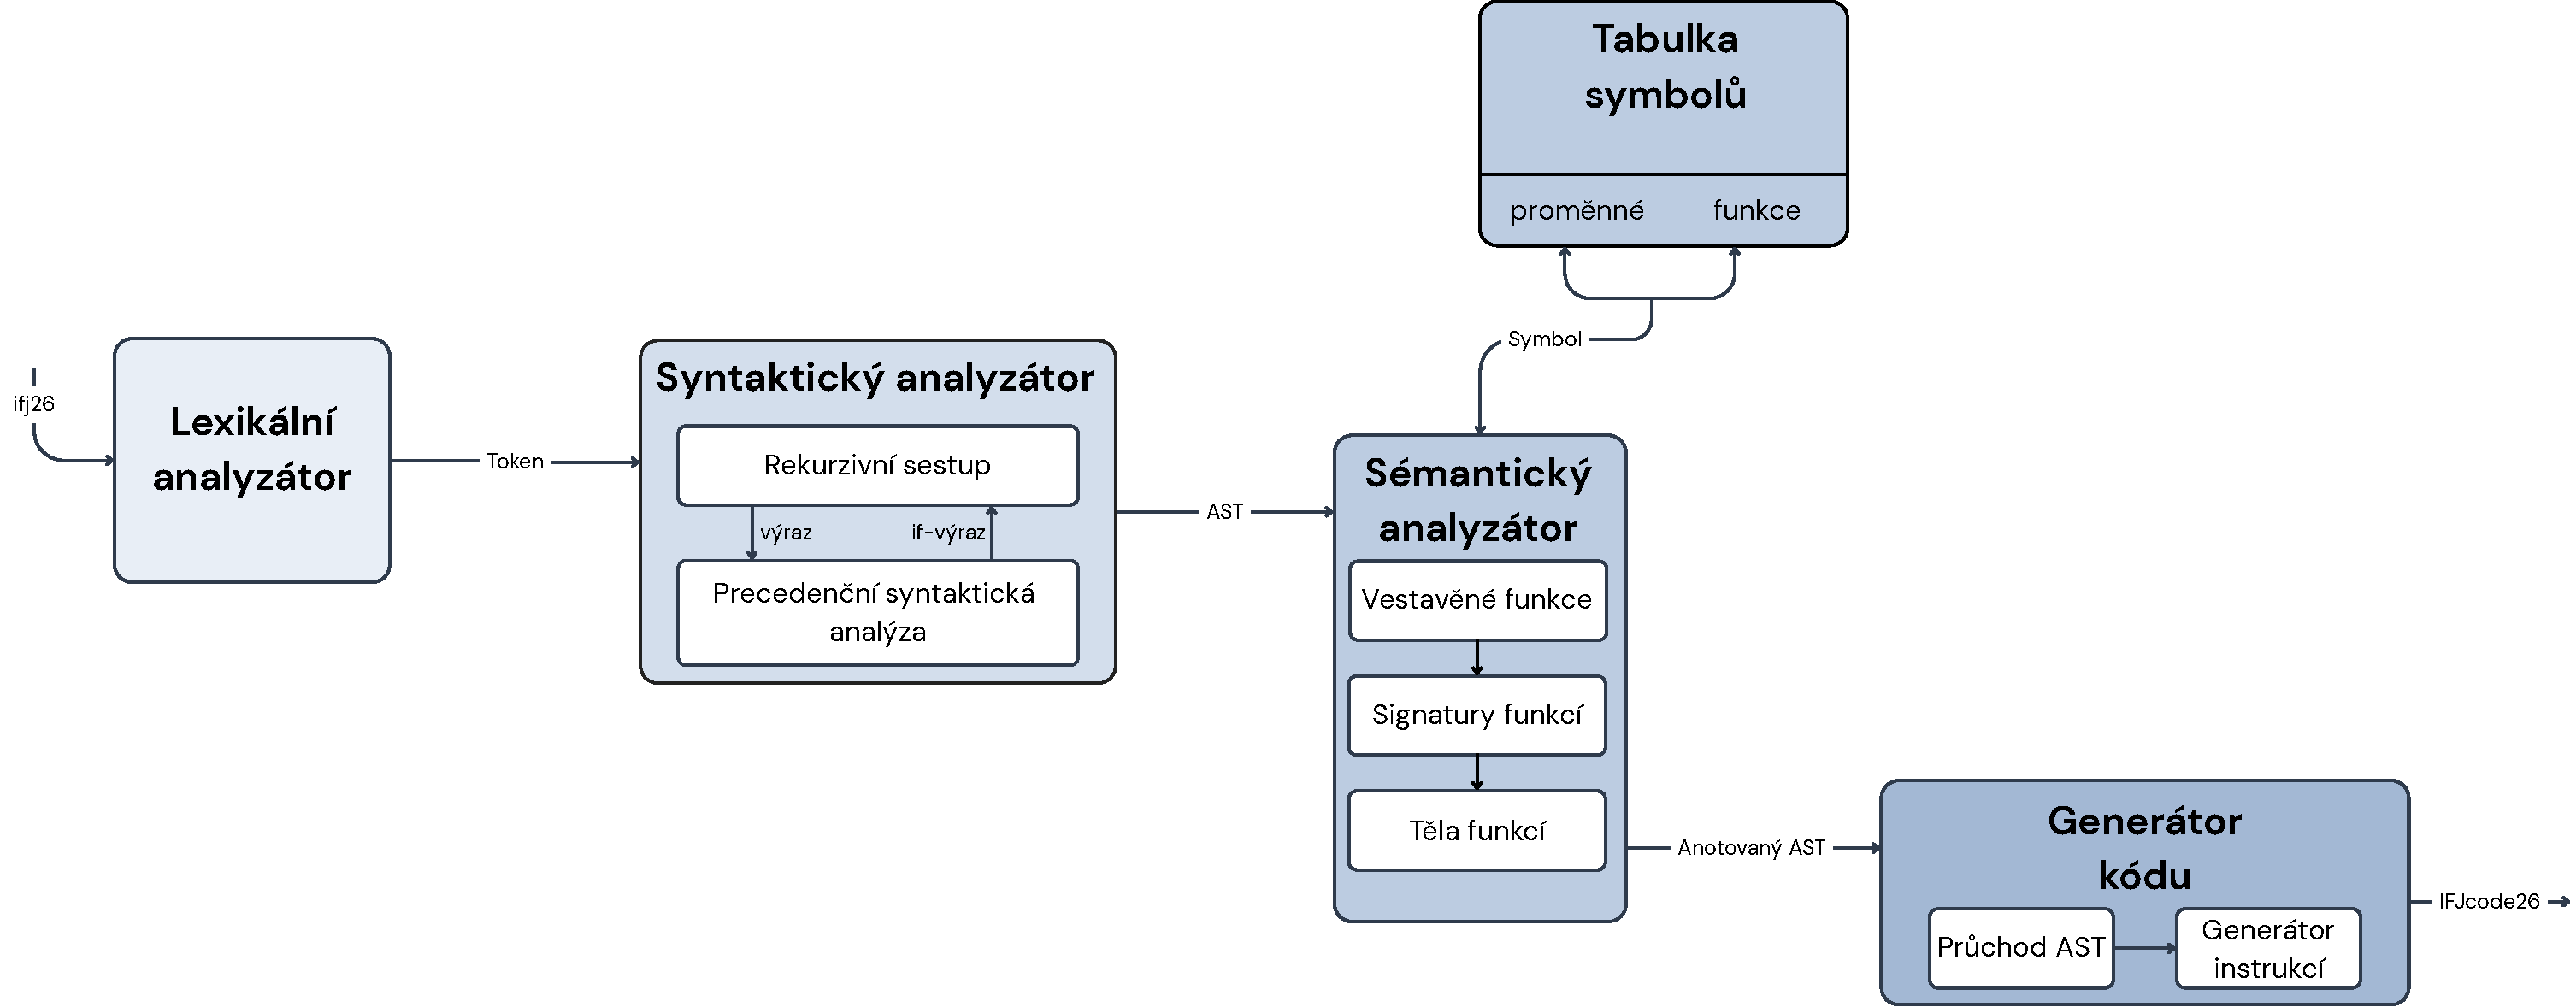
\includegraphics[width=\linewidth]{obrazky/architektura.pdf}
  \fbox{\parbox[c][6cm][c]{0.9\linewidth}{\centering
    \TODOinline{doplnit}}}
  \caption{Blokové schéma překladače a datové toky mezi moduly}
  \label{fig:architektura}
\end{figure}

\TODO{Jak jdou data mezi moduly (tokeny, AST, IFJcode26) a kolik je průchodů?}

% =====================================================================
%  Lexikální analýza
% =====================================================================
\section{Lexikální analýza}\label{sec:lexer}

\subsubsection*{Popis automatu}
Lexer implementuje konečný automat viditelný na obrázcích~\ref{fig:ka-id}
až~\ref{fig:ka-retezce}, které mají společný počáteční stav \texttt{s}.
Stavy \texttt{q} nepřijímající, stavy \texttt{f} přijímající a stavy
\texttt{p} pro zpracování komentáře. Lexer čte nejdelší platný lexém. Když
skončí v~přijímajícím stavu, vrátí token a nepoužitý znak nechá pro další
volání. Neplatný přechod z~nepřijímajícího stavu je lexikální chyba
s~návratovým kódem 1.

\subsubsection*{Odchylka: Vnořené komentáře}
Blokové komentáře lze libovolně vnořovat, což konečný automat sám rozpoznat
nedokáže. Stav \texttt{p2} proto používá čítač \texttt{depth}: \texttt{/*} ho
zvýší, \texttt{*/} sníží a při nule komentář končí. Neuzavřený komentář je
lexikální chyba.

\subsubsection*{Odchylka: Dopředné čtení}
Lexer drží aktuální znak \texttt{current} a jeden znak dopředu,
\texttt{lookahead}. Díky němu rozliší desetinnou tečku od samostatného tokenu
(\texttt{1.5} oproti \texttt{1.foo}) a v~komentářích pozná dvojice
\texttt{/*} a \texttt{*/}.

\subsubsection*{Odchylka: Dodatečná validace}
Po přečtení identifikátoru rozhodne funkce \texttt{keyword()}, jestli jde
o~klíčové nebo rezervované slovo. U~číselných literálů lexer kontroluje
počáteční nuly a pomocí \texttt{strtod} rozsah typu \texttt{Double}. Hlídá
i~hranice tokenů, třeba když za číslem nebo \texttt{@main} pokračuje znak
identifikátoru. Původní zápis lexému se nemění.

\subsubsection*{Odchylka: Logické řádky a odsazení}
Bílé znaky, komentáře a odsazení zpracovává lexer mimo samotný automat.
\texttt{TOKEN\_NEWLINE} vrací jen na konci neprázdného logického řádku mimo
závorky. Kontroluje pokračování řádků, tabulátory v~odsazení a pravidla pro
víceřádkové komentáře. Tokeny \texttt{INDENT} a \texttt{DEDENT} nepoužívá,
parser dostane odsazení a příznak na začátku řádku přímo ve struktuře
\texttt{token\_t}.

% diagramy v TikZu: obrazky/ka-*.tex (všechny začínají ve stavu s)

\begin{figure}[htbp]
  \centering
  % KA lexeru -- identifikátory, klíčová slova, @main, samotné _
\begin{tikzpicture}[ka,px]
  \node[state,initial]   (s)   at (208,266)  {$s$};
  \node[state,accepting] (f31) at (458,147)  {$f_{31}$};
  \node[state,accepting] (f1)  at (818,266)  {$f_{1}$};
  \node[state]           (q2)  at (408,430)  {$q_{2}$};
  \node[state]           (q3)  at (628,430)  {$q_{3}$};
  \node[state]           (q4)  at (848,430)  {$q_{4}$};
  \node[state]           (q5)  at (1068,430) {$q_{5}$};
  \node[state,accepting] (f2)  at (1288,430) {$f_{2}$};

  \node[tok,below=0.5mm of f31]            {TOKEN\_UNDERSCORE};
  \node[tok,below=1mm of f1,align=center]  {TOKEN\_IDENTIFIER\\/ klíčové slovo};
  \node[tok,below=1mm of f2]               {TOKEN\_MAIN};

  \draw[hrana] (s) -- (320,266) |- node[lbl,above,pos=0.75] {\kaPod} (f31);
  \draw[hrana] (s) -- node[lbl,below,pos=0.5] {\kaPis} (f1);
  \draw[hrana] (f31) -| (712,266) -- (f1);
  \node[lbl,above right] at (500,147) {\kaPis\,+\,\kaCis\,+\,\kaPod};
  \path (f1) edge[loop right] node[right] {\kaPis\,+\,\kaCis\,+\,\kaPod} ();
  \draw[hrana] (s) |- node[lbl,above,pos=0.75] {\texttt{@}} (q2);
  \draw[hrana] (q2) -- node[lbl,above] {\texttt{m}} (q3);
  \draw[hrana] (q3) -- node[lbl,above] {\texttt{a}} (q4);
  \draw[hrana] (q4) -- node[lbl,above] {\texttt{i}} (q5);
  \draw[hrana] (q5) -- node[lbl,above] {\texttt{n}} (f2);
\end{tikzpicture}

  \caption{Konečný automat lexeru -- identifikátory, klíčová slova
           a \texttt{@main}}
  \label{fig:ka-id}
\end{figure}

\begin{figure}[htbp]
  \centering
  % KA lexeru -- komentáře (rozšíření o čítač depth)
\begin{tikzpicture}[ka,px]
  \node[state,initial]   (s)   at (88,300)  {$s$};
  \node[state,accepting] (f26) at (338,300) {$f_{26}$};
  \node[state]           (p1)  at (638,300) {$p_{1}$};
  \node[state]           (p2)  at (638,560) {$p_{2}$};

  \node[tok, below=1mm of f26] {TOKEN\_SLASH};
  \node[pozn,below=1mm of p1]  {řádkový komentář};
  \node[pozn,below=1mm of p2]  {blokový komentář};

  \draw[hrana] (s) -- node[lbl,above] {\texttt{/}} (f26);
  \draw[hrana] (f26.east) -- (462,300) |- node[lbl,above,pos=0.75] {\texttt{/}} (p1);
  \path (p1) edge[loop right] node[lbl,right=1pt] {\kaKrome{LF}} ();
  \draw[hrana] (p1) |- node[lbl,above,pos=0.75] {LF / zpracuj konec řádku} (88,155) -- (s);
  \draw[hrana] (f26.east) -- (462,300) |- (p2);
  \node[lbl,left] at (462,485) {\texttt{*} / $\mathit{depth}=1$};
  \path (p2) edge[loop above] node[lbl] {\texttt{/*} / $\mathit{depth}{+}{+}$} ();
  \path (p2) edge[loop right] node[lbl,right=2pt] {\texttt{*/} a $\mathit{depth}>1$ / $\mathit{depth}{-}{-}$} ();
  \draw[hrana] (p2.west) -- (492,560) |- (492,720) -| (s);
  \node[lbl,below] at (290,720) {\texttt{*/} a $\mathit{depth}=1$ / $\mathit{depth}{-}{-}$; dokonči komentář};
\end{tikzpicture}

  \caption{Konečný automat lexeru -- komentáře
           (rozšíření o~čítač $\mathit{depth}$)}
  \label{fig:ka-komentare}
\end{figure}

\begin{figure}[htbp]
  \centering
  % KA lexeru -- operátory a oddělovače
% oba uzly s = tentýž stav
\begin{tikzpicture}[ka,px,every state/.append style={minimum size=7.5mm}]
  % --- levá část: jednoznakové tokeny ---------------------------------
  \node[state,initial] (s) at (88,616) {$s$};
  \foreach \i/\id/\sym/\tk/\x in {
      0/3/(/LPAREN/180,  1/4/)/RPAREN/193,  2/5/:/COLON/207,
      3/6/{,}/COMMA/221, 4/7/;/SEMICOLON/235, 5/8/+/PLUS/249,
      6/9/-/MINUS/263,   7/10/*/STAR/277,   8/33/[/LBRACKET/291,
      9/34/]/RBRACKET/305, 10/35/\{/LBRACE/319, 11/36/\}/RBRACE/333} {
    \node[state,accepting] (f\id) at (448,236+110*\i) {$f_{\id}$};
    % popisky vpravo od stavů
    \node[tok,right=0.5mm of f\id] {TOKEN\_\tk};
    \draw[hrana] (s.east) -- (\x,616) |- (f\id);
    \node[lbl,above] at (362,236+110*\i) {\texttt{\sym}};
  }

  % --- pravá část: víceznakové operátory -----------------------------
  \node[state,initial] (t)   at (838,616)   {$s$};
  \node[state,accepting] (f11) at (1138,276)  {$f_{11}$};
  \node[state,accepting] (f14) at (1438,276)  {$f_{14}$};
  \node[state,accepting] (f12) at (1138,496)  {$f_{12}$};
  \node[state,accepting] (f15) at (1438,496)  {$f_{15}$};
  \node[state,accepting] (f30) at (1438,606)  {$f_{30}$};
  \node[state,accepting] (f13) at (1138,716)  {$f_{13}$};
  \node[state,accepting] (f16) at (1438,716)  {$f_{16}$};
  \node[state,accepting] (f27) at (1138,936)  {$f_{27}$};
  \node[state,accepting] (f17) at (1438,936)  {$f_{17}$};
  \node[state]           (q19) at (1138,1066) {$q_{19}$};
  \node[state,accepting] (f28) at (1438,1066) {$f_{28}$};
  \node[state,accepting] (f32) at (1138,1196) {$f_{32}$};
  \node[state,accepting] (f29) at (1438,1196) {$f_{29}$};

  \foreach \n/\tk in {f11/ASSIGN, f14/EQUAL, f12/LESS, f15/LESS\_EQUAL,
                      f30/LARROW, f13/GREATER, f16/GREATER\_EQUAL,
                      f27/NOT, f17/NOT\_EQUAL, f28/AND, f32/PIPE, f29/OR}
    \node[tok,below=0.2mm of \n] {TOKEN\_\tk};
  \node[pozn,below=0.2mm of q19,xshift=4mm] {samotné \& je chyba};

  \foreach \n/\sym/\x in {f11/=/930, f12/</944, f13/>/958, f27/!/972,
                          q19/\&/990, f32/|/1010}
    \draw[hrana] (t.east) -- (\x,616) |-
      node[lbl,above,pos=0.8] {\texttt{\sym}} (\n);
  \draw[hrana] (f11) -- node[lbl,above] {\texttt{=}} (f14);
  \draw[hrana] (f12) -- node[lbl,above] {\texttt{=}} (f15);
  \draw[hrana] (f12.east) -- (1252,496) |- node[lbl,above,pos=0.75] {\texttt{-}} (f30);
  \draw[hrana] (f13) -- node[lbl,above] {\texttt{=}} (f16);
  \draw[hrana] (f27) -- node[lbl,above] {\texttt{=}} (f17);
  \draw[hrana] (q19) -- node[lbl,above] {\texttt{\&}} (f28);
  \draw[hrana] (f32) -- node[lbl,above] {\texttt{|}} (f29);
\end{tikzpicture}

  \caption{Konečný automat lexeru -- operátory a oddělovače
           (oba uzly $s$ jsou tentýž počáteční stav)}
  \label{fig:ka-op}
\end{figure}

\begin{figure}[htbp]
  \centering
  % KA lexeru -- číselné literály a tečka
\begin{tikzpicture}[ka,px]
  \node[state,initial]   (s)   at (96,467)   {$s$};
  \node[state,accepting] (f22) at (96,277)   {$f_{22}$};
  \node[state,accepting] (f18) at (376,467)  {$f_{18}$};
  \node[state]           (q7)  at (376,706)  {$q_{7}$};
  \node[state]           (q8)  at (676,467)  {$q_{8}$};
  \node[state,accepting] (f19) at (976,467)  {$f_{19}$};
  \node[state]           (q9)  at (976,706)  {$q_{9}$};
  \node[state,accepting] (f21) at (1276,467) {$f_{21}$};
  \node[state]           (q12) at (1276,677) {$q_{12}$};
  \node[state]           (q10) at (676,906)  {$q_{10}$};
  \node[state]           (q11) at (976,906)  {$q_{11}$};
  \node[state,accepting] (f20) at (1276,906) {$f_{20}$};

  \node[tok,above=1mm of f22]  {TOKEN\_DOT};
  \node[tok,below=1mm of f18]  {TOKEN\_INTEGER};
  \node[tok,below=1mm of f19]  {TOKEN\_DOUBLE};
  \node[tok,below=1mm of f21]  {TOKEN\_DOUBLE};
  \node[tok,anchor=north west] at (f20.south east) {TOKEN\_DOUBLE};
  \node[pozn,below=1mm of q7,align=center]  {po \kaPod{} je\\nutná číslice};
  \node[pozn,below=1mm of q8,align=center]  {nutná desetinná\\číslice};
  \node[pozn,below=1mm of q9,align=center]  {po \kaPod{} je\\nutná číslice};
  \node[pozn,below=0.5mm of q12,align=center] {po \kaPod{} je\\nutná číslice};
  \node[pozn,anchor=north east,align=right] at (q10.south west) {za \texttt{e}/\texttt{E}\\musí být číslice};
  \node[pozn,below=1mm of q11,align=center] {po znaménku\\číslice};

  % s
  \draw[hrana] (s) -- node[lbl,above] {\kaCis} (f18);
  \draw[hrana] (s) -- node[lbl,left] {\large\texttt{.}} (f22);
  \draw[hrana] (f22) -| node[lbl,above,pos=0.25] {\kaCis} (f19);
  % celá část
  \path (f18) edge[loop above] node[lbl] {\kaCis} ();
  \draw[hrana] (f18.east) -- (492,467) |- (q7);
  \node[lbl,above] at (462,467) {\kaPod};
  \draw[hrana] (q7) -- (245,706) |- node[lbl,left,pos=0.25] {\kaCis} (f18);
  \path (q7) edge[loop above] node[lbl] {\kaPod} ();
  \draw[hrana] (f18) -- node[lbl,above,pos=0.8] {\large\texttt{.}} (q8);
  \draw[hrana] (f18.east) -- (530,467) |- (q10);
  \node[lbl,right] at (530,620) {\texttt{e}\,+\,\texttt{E}};
  % desetinná část
  \draw[hrana] (q8) -- node[lbl,above,pos=0.35] {\kaCis} (f19);
  \path (f19) edge[out=115,in=160,looseness=7] node[lbl,above] {\kaCis} (f19);
  \draw[hrana] (f19.east) -- (1092,467) |- (q9);
  \node[lbl,above] at (1050,467) {\kaPod};
  \draw[hrana] (q9) -- (845,706) |- node[lbl,left,pos=0.25] {\kaCis} (f19);
  \path (q9) edge[loop above] node[lbl] {\kaPod} ();
  \draw[hrana] (f19) -- node[lbl,above,pos=0.7] {\texttt{d}\,+\,\texttt{D}} (f21);
  \draw[hrana] (f19.east) -- (1110,467) |- (1110,828) -| (q10);
  \node[lbl,above] at (780,828) {\texttt{e}\,+\,\texttt{E}};
  % exponent
  \draw[hrana] (q10) -- node[lbl,above] {\texttt{+}\,+\,\texttt{-}} (q11);
  \draw[hrana] (q11) -- node[lbl,above] {\kaCis} (f20);
  \draw[hrana] (q10) |- (676,1080) -| node[lbl,above,pos=0.25] {\kaCis} (f20);
  \path (f20) edge[loop above] node[lbl] {\kaCis} ();
  \draw[hrana] (f20.west) -- (1160,906) |- (q12);
  \node[lbl,left] at (1160,800) {\kaPod};
  \draw[hrana] (q12) -- (1430,677) |- node[lbl,left,pos=0.25] {\kaCis} (f20);
  \path (q12) edge[loop above] node[lbl] {\kaPod} ();
  \draw[hrana] (f20.east) -- (1520,906) |- node[lbl,right,pos=0.25] {\texttt{d}\,+\,\texttt{D}} (f21);
\end{tikzpicture}

  \caption{Konečný automat lexeru -- číselné literály a tečka}
  \label{fig:ka-cisla}
\end{figure}

\begin{figure}[htbp]
  \centering
  % KA lexeru -- běžné a víceřádkové řetězce
\begin{tikzpicture}[ka,px]
  \node[state,initial]   (s)   at (96,377)   {$s$};
  \node[state]           (q13) at (346,377)  {$q_{13}$};
  \node[state,accepting] (f23) at (646,377)  {$f_{23}$};
  \node[state]           (q16) at (946,377)  {$q_{16}$};
  \node[state]           (q17) at (1196,377) {$q_{17}$};
  \node[state]           (q18) at (1446,377) {$q_{18}$};
  \node[state,accepting] (f25) at (1446,587) {$f_{25}$};
  \node[state]           (q14) at (346,687)  {$q_{14}$};
  \node[state]           (q15) at (646,687)  {$q_{15}$};
  \node[state,accepting] (f24) at (96,877)   {$f_{24}$};

  \node[pozn,below=1mm of q13]                 {první uvozovka};
  \node[tok, below=1mm of f23]                 {TOKEN\_STRING: \kaUv\kaUv};
  \node[pozn,anchor=north west,align=left] at (q16.south east) {raw: žádná\\závěrečná \kaUv};
  \node[pozn,anchor=north west,align=left] at (q17.south east) {raw: jedna\\závěrečná \kaUv};
  \node[pozn,anchor=south west,align=left] at (q18.north east) {raw: dvě\\závěrečné \kaUv};
  \node[tok, below=1mm of f25]                 {TOKEN\_STRING};
  \node[pozn,anchor=north west,align=left] at (q14.south east) {obsah běžného\\řetězce};
  \node[pozn,right=1mm of q15]                 {escape};
  \node[tok, below=1mm of f24]                 {TOKEN\_STRING};

  % běžný řetězec
  \draw[hrana] (s) -- node[lbl,above,pos=0.3] {\kaUv} (q13);
  \draw[hrana] (q13) -- node[lbl,above] {\kaUv} (f23);
  \draw[hrana] (q13.west) -- (228,377) |- (q14);
  \node[lbl,left,align=right] at (228,540) {\kaKrome{\kaUv\,+\,\kaBs\\+\,LF}};
  \path (q14) edge[loop above] ();
  \node[lbl,right] at (360,610) {\kaKrome{\kaUv\,+\,\kaBs\,+\,LF}};
  \draw[hrana] (q13.east) -- (470,377) |- (470,490) -| (q15);
  \node[lbl,below] at (560,490) {\kaBs};
  \draw[hrana] (q14) -- node[lbl,above] {\kaBs} (q15);
  \draw[hrana] (q15) |- (346,858) -- (q14);
  \node[lbl,above] at (496,858) {\kaBs\,+\,\kaUv\,+\,\texttt{n}\,+\,\texttt{r}\,+\,\texttt{t}};
  \draw[hrana] (q14.west) -- (96,687) -- node[lbl,left,pos=0.5] {\kaUv} (f24);
  % víceřádkový řetězec
  \draw[hrana] (f23) -- node[lbl,above] {\kaUv} (q16);
  \path (q16) edge[out=110,in=150,looseness=7] node[lbl,left] {\kaKrome{\kaUv}} (q16);
  \draw[hrana] (q16) -- node[lbl,above] {\kaUv} (q17);
  \draw[hrana] (q17) -- node[lbl,above] {\kaUv} (q18);
  \draw[hrana] (q17) |- (946,545) -- (q16);
  \node[lbl,below] at (1071,545) {\kaKrome{\kaUv}};
  \draw[hrana] (q18) |- (946,195) -- (q16);
  \node[lbl,above] at (1196,195) {\kaKrome{\kaUv}};
  \draw[hrana] (q18.east) -- (1560,377) |- node[lbl,right,pos=0.25] {\kaUv} (f25);
  \path (f25) edge[loop left] node[lbl] {\kaUv} ();
\end{tikzpicture}

  \caption{Konečný automat lexeru -- běžné a víceřádkové řetězce}
  \label{fig:ka-retezce}
\end{figure}

% =====================================================================
%  Syntaktická analýza
% =====================================================================
\section{Syntaktická analýza}\label{sec:parser}

\subsection{Rekurzivní sestup}\label{sec:rek-sestup}
\TODO{Odpovídá parser gramatice funkcí na neterminál? Kolik tokenů čte dopředu?}

\subsection{Precedenční analýza výrazů}\label{sec:precedence}
\TODO{Kdy parser předává řízení precedenční analýze a jak se vrací?}

% --- precedenční tabulka ---------------------------------------------
% \shift <  \reduce >  \equal =  prázdná buňka = chyba
\begin{table}[H]
  \centering
  \renewcommand{\arraystretch}{1.2}
  \begin{tabular}{c|cccc}
           & \TODOinline{op} & \texttt{(} & \texttt{)} & \$ \\ \hline
    \TODOinline{op} & & & & \\
    \texttt{(}      & & & & \\
    \texttt{)}      & & & & \\
    \$              & & & & \\
  \end{tabular}
  \caption{Precedenční tabulka (řádek = terminál na zásobníku,
           sloupec = vstupní token)}
  \label{tab:precedence}
\end{table}

\subsection{Sémantická analýza}\label{sec:semantika}
Pro provedení sémantické analýzy se volá funkce \texttt{semantic\_analyze}.
\begin{itemize}[nosep]
  \item Pass 0: Přidá všechny vestavěné funkce do tabulky symbolů.
  \item Pass 1: Projde všechny funkce a přidá je do tabulky symbolů.
  \item Pass 2: Projde tělo každé funkce a provede sémantickou analýzu,
        včetně kontroly pravidel, typových kontrol, typových konverzí,
        kompatibility typů a odvozování typů. Zároveň do AST doplní
        informace potřebné pro codegen.
\end{itemize}

\TODO{Něco doplnit k průchodům, třeba val a var nebo návratové typy?}

\subsection{Generování cílového kódu}\label{sec:codegen}
\TODO{Jak se řeší rámce, návěští a vestavěné funkce?}

\section{Sémantická analýza}\label{sec:semantika}
Pro provedení sémantické analýzy se volá funkce \texttt{semantic\_analyze}.
\begin{itemize}[nosep]
  \item Pass 0: Přidá všechny vestavěné funkce do tabulky symbolů.
  \item Pass 1: Projde všechny funkce a přidá je do tabulky symbolů.
  \item Pass 2: Projde tělo každé funkce a provede sémantickou analýzu,
        včetně kontroly pravidel, typových kontrol, typových konverzí,
        kompatibility typů a odvozování typů. Zároveň do AST doplní
        informace potřebné pro codegen.
\end{itemize}

\TODO{Něco doplnit k průchodům, třeba val a var nebo návratové typy?}

\section{Generování cílového kódu}\label{sec:codegen}
\TODO{Jak se řeší rámce, návěští a vestavěné funkce?}

% =====================================================================
%  Tabulka symbolů
% =====================================================================
\section{Tabulka symbolů}\label{sec:symtable}

Na základě vybrané varianty vv-BVS jsme museli tabulku symbolů implementovat jako výškově vyvážený binární
vyhledávací strom (zvolili jsme AVL strom~\cite{ial06vyhledavani}). Klíčem do tabulky symbolů je jméno identifkátoru, uzly se řadí lexikograficky
pomocí \fce{strcmp}.

\subsection{Struktura}
Funkce a proměnné jsou uloženy v~tabulce symbolů odděleně. Funkce (uživatelské i~vestavěné) jsou v~jednom globálním
stromu, protože jsou viditelné pro celý program. Proměnné se ukládají do zásobníku rozsahů, který je implementován
jako jednosměrně vázaný seznam. Každý rozsah by měl odpovídat jednomu bloku zdrojového kódu
(má vlastní strom a hloubku na zásobníku). Sémantická analýza vždy při vstupu do bloku vloží rozsah (\fce{symtable\_push\_scope}) a když jej opouští, volá se
\fce{symtable\_pop\_scope}.

\subsection{Obsah symbolu}
Každý uzel obsahuje strukturu \texttt{symbol\_t}. U~proměnné obsahuje typ, příznak konstanty a jedinečný identifikátor. U~funkce symbol obsahuje navíc ještě návratový typ,
typy a jména parametrů, příznak vestavěné funkce, příznak \texttt{@main}, stav kontroly těla (kapitola~\ref{sec:semantika}) a příznak odvození
návratového typu a ukazatel na definici funkce v~AST.

\subsection{Operace se stromem}
Vkládaní probíhá rekurzivně sestupem. Když se z~rekurze vrací, přepočítá se výška a strom se případně vyváží na základě rozdílu výšek podstromů.
Vyvážení se provádí aplikací jedné ze čtyř možných rotací (LL, LR, RL, RR). Když uzel se stejným klíčem už existuje, funkce která vkládaní provádí,
vrátí \texttt{ST\_EXISTS}. V~sémantice se z toho stane chyba~4.

Vyhledávání probíhá následovně: proměnná se hledá od vrcholu zásobníku směrem dolů a
vratí se první nalezená hodnota - ta z nejvnitřnějšího bloku (funguje tak zastíňení). Pro kontrolu redefinice prohledá funkce \fce{symtable\_lookup\_local} jen aktuální rozsah.

Proměnné zanikají vždy s~celým blokem (při odstranění rozsahu se uvolňuje celý jeho strom).
Vkládaní i~vyhledávání má časovou složitost $O(\log n)$.

Součástí tabulky symbolů je taky čítač, který přiřazuje jedinečná čísla symbolům.
Vkládaní vrací ukazatel na vložený symbol, aby ho volající mohl hned doplnit.


% =====================================================================
%  Popis modulů
%  Tady se to snažte držet skromně dle zadání jedna věta stačí.
% =====================================================================
\section{Popis modulů}\label{sec:moduly}

\begin{description}[style=nextline]
  \item[\texttt{ast.c/.h}]
    Obsahuje deklarace všech uzlů abstraktního syntaktického stromu (AST)
    a deklarace jejich konstruktorů. Implementuje konstruktory pro všechny
    typy uzlů AST. Součástí je také funkce pro výpis AST, vygenerovaná
    pomocí AI, která slouží k~ladění programu.
  \item[\texttt{codegen.c/.h}]              \TODOinline{...}
  \item[\texttt{codegen\_ast.c/.h}]         \TODOinline{...}
  \item[\texttt{comp\_error.h}]             \TODOinline{...}
  \item[\texttt{dynamic\_array.c/.h}]       \TODOinline{...}
  \item[\texttt{lexer.c/.h}]
    Provádí lexikální analýzu dle diagramu automatu. Samostatné funkce čtou
    identifikátory, operátory, čísla, řetězce a komentáře, pomocné funkce
    kontrolují literály, logické řádky, odsazení a hlásí případné chyby.
  \item[\texttt{main.c}]
    Načítá zdrojový kód ze standardního vstupu (\texttt{stdin}) a vypisuje
    vygenerovaný kód IFJcode26 na standardní výstup (\texttt{stdout}).
  \item[\texttt{parser.c/.h}]               Implementuje syntaktický analyzátor řízený rekurzivním sestupem. Zpracovává hlavičku, definice funkcí, vstupní bod, vnořené bloky řízené odsazením, deklarace proměnných, přiřazení i řídicí konstrukce a sestavuje AST, a hlásí případné chzbz.
  \item[\texttt{parser\_expression.c/.h}]   \TODOinline{...}
  \item[\texttt{parser\_stack.h}]           \TODOinline{...}
  \item[\texttt{semantic.c/.h}]
    Jedinou funkcí, která by se z~tohoto modulu \textbf{měla používat},
    je \texttt{semantic\_analyze}, která provádí sémantickou analýzu AST
    předaného programu.
  \item[\texttt{symtable.c/.h}]
    Proměnné jsou uloženy v~zásobníku oblastí platnosti (scope), přičemž
    každá oblast je reprezentována jedním binárním vyhledávacím stromem
    (BST). Funkce jsou uloženy v~globálním binárním vyhledávacím stromu
    (BST).
  \item[\texttt{test\_lexer.c}]
    Regresní testy lexeru. Obsahuje platné i~neplatné vstupy, hraniční
    případy, rozšíření jazyka a kontrola správy paměti.
  \item[\texttt{token.h}]
    Zajišťuje typy tokenů a strukturu \texttt{token\_t}, kterou sdílí lexer
    s~parserem. Nese typ tokenu, původní lexém a jeho délku, pozici ve
    zdrojovém souboru, odsazení a příznak začátku logického řádku.
  \item[\texttt{types.c/.h}]                \TODOinline{...}
  \item[\texttt{utils.c/.h}]
    Alokuje paměť pro řetězec (\texttt{str}) a vrací jeho kopii, která je
    uložena na haldě (heap).
\end{description}

% =====================================================================
%  Využití AI
% =====================================================================
\section{Využití nástrojů AI}\label{sec:ai}

\subsection{Použité nástroje a modely}
% počty = kolik jsem našel AI labels v kódech všech
\begin{center}
\small
\begin{tabular}{@{}l l p{7.2cm}@{}}
  \toprule
  \textbf{Člen} & \textbf{Nástroj / model} & \textbf{Kde (označené segmenty)} \\
  \midrule
  Dušan Popović   & Gemini / Gemini 4 HYDROGEN
                  & komentáře v~\texttt{parser.h}, \texttt{parser\_expression.h},
                    pomocné funkce parseru, testy parseru \\
                  & Claude / Claude Sonnet 5.5
                  & pomocné funkce v~\texttt{parser.c} \\
  \addlinespace
  Marek Záchenský & Claude Code / Claude Opus 5.5
                  & komentáře v~\texttt{codegen.h}, \texttt{codegen\_ast.h},
                    testy generátoru, end-to-end testy (\texttt{tests/e2e}) \\
  \addlinespace
  Adam Zatloukal  & Claude Code / Claude Opus 5.5
                  & pomocná makra a funkce v~\texttt{ast}, \texttt{dynamic\_array},
                    \texttt{types}, \texttt{utils}, \texttt{comp\_error.h},
                    \texttt{.clang-format}, makra pro inicializaci
                    \texttt{symbol\_t}, testy AST, tabulky symbolů a sémantiky \\
                  & Claude Code / Claude Fable 5.2
                  & část pro BOOLTHEN (\texttt{ast.c}, testy sémantiky) \\
  \addlinespace
  Tadeáš Zonyga   & Claude Code / Claude Opus 5.5
                  & části \texttt{lexer.c} implementované podle vlastního
                    diagramu automatu, testy lexeru \\
                  & Codex CLI / GPT-6 Astra (Medium)
                  & rozšíření testů lexeru (řetězce, komentáře, chyby,
                    logické řádky, celé programy) \\
  \bottomrule
\end{tabular}
\end{center}

\subsection{Pracovní postup}
Tadeáš: AI jsem se při práci na lexeru pokoušel využíval skoro v~každé části
projektu kromě samotného návrhu konečného automatu. I~tam jsem ale s~pomocí
AI vytvořil vlastní nástroj pro návrh automatů, ve kterém jsem automat
skládal z~jednotlivých dílků jako LEGO a hned viděl, jak jím budou procházet
jednotlivé vstupy viz. obrázek \TODOinline{ten ještě musím doplnit}. Z~tohoto
nástroje jsme pak postavili i~interaktivní vizualizaci pro kolegy dostupnou
zde \url{https://ifj26-lexer.zonyga-tadeas.workers.dev/}. Nejvíc mi AI
pomohla při code review, při implementaci podle mého diagramu a při psaní
regresních testů. Diagram jsem nejdřív převedl do podrobného zadání pro AI,
následně se mě ptala na doplňující otázky pro upřesnění jednotlivých
pravidel, na jejichž základě jsme pak psali samotný kód.

\TODO{VŠICHNI: Uhladit. K čemu jste AI typicky používali?}

\subsection{Problémy a odmítnuté návrhy}
Tadeáš: Při rozšiřování testů AI (konkrétně GPT-6 Astra) začala upravovat
implementaci lexeru, aby nové testy, které měla napsat, procházely. Místo
toho mě měla upozornit na neprocházejíci testy dle instrukcí v~promptu. Tyto
změny jsem odmítl, kód vrátil a diagram upravil sám, aby nové testy taky
procházely.

\TODO{VŠICHNI: Uhladit. Kdy vám AI poradila špatně?}

\subsection{Kde jsme AI nepoužili}
Konečný automat lexeru a pravidla pro rozpoznávání tokenů jsme navrhli sami.
AI jsme použili až na vizualizaci (o~čem mluvil Tadeáš), kontrolu přechodů
a převod návrhu do kódu.

\TODO{VŠICHNI: Uhladit. Kde jste AI nepoužili? Je strom bez AI (AI jsou jen makra pro symbol\_t)?}


% --- literatura -------------------------------------------------------
\bibliographystyle{plainurl}
\bibliography{literatura}

% --- přílohy ----------------------------------------------------------
\appendix
% =====================================================================
%  Příloha A: LL gramatika a LL tabulka (bez AI)
% =====================================================================
\section{LL gramatika}\label{app:gramatika}



\begin{gramatika}
  
    \item \verb|<prog> -> import ifj26 . * EOL <top_list> EOF|
    \item \verb|<top_list> -> <top_item> <top_list>|
    \item \verb|<top_list> -> |$\varepsilon$
    \item \verb|<top_item> -> @main EOL <main_def>|
    \item \verb|<top_item> -> <func_def>|
    \item \verb|<main_def> -> def main () : Unit = <func_body>|
    \item \verb|<func_def> -> def id (<param_list>) : <type> = <func_body>|
    \item \verb|<param_list> -> <param> <param_tail>|
    \item \verb|<param_list> -> |$\varepsilon$
    \item \verb|<param_tail> -> , <param_next>|
    \item \verb|<param_tail> -> |$\varepsilon$
    \item \verb|<param_next> -> <param> <param_tail>|
    \item \verb|<param_next> -> |$\varepsilon$
    \item \verb|<param> -> id : <type>|
    \item \verb|<type> -> Int|
    \item \verb|<type> -> Double|
    \item \verb|<type> -> String|
    \item \verb|<type> -> Boolean|
    \item \verb|<type> -> Unit|
    \item \verb|<func_body> -> EOL INDENT <stmt_list> DEDENT|
    \item \verb|<func_body> -> <expr> EOL|
    \item \verb|<stmt_list> -> <stmt> <stmt_list>|
    \item \verb|<stmt_list> -> |$\varepsilon$|
    \item \verb|<stmt> -> val id <opt_type> = <expr> EOL|
    \item \verb|<stmt> -> var id <opt_type> = <expr> EOL|
    \item \verb|<stmt> -> <func_def>|
    \item \verb|<stmt> -> while (<expr>) do <block>|
    \item \verb|<stmt> -> for (id <- <expr> <range_op> <expr> <opt_by>) do <block>|
    \item \verb|<stmt> -> return <opt_expr> EOL|
    \item \verb|<stmt> -> <expr> <stmt_assign> EOL|
    \item \verb|<opt_type> -> : <type>|
    \item \verb|<opt_type> -> |$\varepsilon$
    \item \verb|<stmt_assign> -> = <expr>|
    \item \verb|<stmt_assign> -> |$\varepsilon$
    \item \verb|<range_op> -> until|
    \item \verb|<range_op> -> to|
    \item \verb|<opt_by> -> by <expr>|
    \item \verb|<opt_by> ->| $\varepsilon$
    \item \verb|<opt_expr> -> <expr>|
    \item \verb|<opt_expr> -> |$\varepsilon$
    \item \verb|<block> -> EOL INDENT <stmt_list> DEDENT| 
\end{gramatika}

% ---------------------------------------------------------------------
\begin{landscape}
\section{LL tabulka}\label{app:ll-tabulka}
 
% řádky = neterminály, sloupce = terminály, buňka = číslo pravidla
\begin{table}[H]
  \centering
  \footnotesize
  \setlength{\tabcolsep}{4pt}
  \renewcommand{\arraystretch}{1.25}
  \setlength{\arrayrulewidth}{0.2pt}
  \begin{tabular}{|l|c|c|c|c|c|c|c|c|c|c|c|c|c|c|c|c|c|c|c|c|}
    \hline
    Neterminál & import & @main & def & id & val & var & while & for & return & type & : & = & , & ) & range & by & expr & EOL & DEDENT & EOF \\ \hline
    <prog> & 1 & & & & & & & & & & & & & & & & & & & \\ \hline
    <top\_list> & & 2 & 2 & & & & & & & & & & & & & & & & & 3 \\ \hline
    <top\_item> & & 4 & 5 & & & & & & & & & & & & & & & & & \\ \hline
    <main\_def> & & & 6 & & & & & & & & & & & & & & & & & \\ \hline
    <func\_def> & & & 7 & & & & & & & & & & & & & & & & & \\ \hline
    <param\_list> & & & & 8 & & & & & & & & & & 9 & & & & & & \\ \hline
    <param\_tail> & & & & & & & & & & & & & 10 & 11 & & & & & & \\ \hline
    <param\_next> & & & & 12 & & & & & & & & & & 13 & & & & & & \\ \hline
    <param> & & & & 14 & & & & & & & & & & & & & & & & \\ \hline
    <type> & & & & & & & & & & 15-19 & & & & & & & & & & \\ \hline
    <func\_body> & & & & 21 & & & & & & & & & & & & & 21 & 20 & & \\ \hline
    <stmt\_list> & & & 22 & 22 & 22 & 22 & 22 & 22 & 22 & & & & & & & & 22 & & 23 & \\ \hline
    <stmt> & & & 26 & 30 & 24 & 25 & 27 & 28 & 29 & & & & & & & & 30 & & & \\ \hline
    <opt\_type> & & & & & & & & & & & 31 & 32 & & & & & & & & \\ \hline
    <stmt\_assign> & & & & & & & & & & & & 33 & & & & & & 34 & & \\ \hline
    <range\_op> & & & & & & & & & & & & & & & 35,36 & & & & & \\ \hline
    <opt\_by> & & & & & & & & & & & & & & 38 & & 37 & & & & \\ \hline
    <opt\_expr> & & & & 39 & & & & & & & & & & & & & 39 & 40 & & \\ \hline
    <block> & & & & & & & & & & & & & & & & & & 41 & & \\ \hline
  \end{tabular}
  \caption{LL tabulka (čísla odkazují na pravidla v~příloze~\ref{app:gramatika})}
  \label{tab:ll}
\end{table}
\end{landscape}


\end{document}
